% ----------------------------------------------------------
\chapter{Tabelas e figuras}
% ----------------------------------------------------------

% ---
\section{Tabelas}
% ---

As \cref{tab:nivel,tab:fluxo,tab:ibge} são exemplos de tabelas construída em
\LaTeX. Observe que a \cref{tab:ibge} utiliza o padrão do \citeonline{ibge1993} para documentos técnicos e acadêmicos.

\begin{table}[htb]
\begin{center}%
\small
\caption[Níveis de investigação]{Níveis de investigação}
\label{tab:nivel}
{\renewcommand{\arraystretch}{1.3} % espaçamento entre as linhas da tabela
\begin{tabular}{p{2.5cm}p{5.4cm}p{2.3cm}p{2.5cm}}
    \rowcolor{verdeunb!10}\textbf{Nível de Investigação} & \textbf{Insumos}  & \textbf{Sistemas de Investigação}  & \textbf{Produtos} \\ \hline
    Meta-nível & Filosofia da Ciência  & Epistemologia & Paradigma \\ \hline
    Nível do objeto & Paradigmas do metanível e evidências do nível inferior & Ciência  & Teorias e modelos \\ \hline
    Nível inferior & Modelos e métodos do nível do objeto e problemas do nível inferior & Prática & Solução de problemas \\
\end{tabular}}
\fonte{\citeonline{van86}}
\end{center}%
\end{table}

\begin{table}[htb]
\small
\begin{center}%
\caption{Componentes curriculares do segundo nível}
\label{tab:fluxo}
{\renewcommand{\arraystretch}{1.3} % espaçamento entre as linhas da tabela
\begin{tabular}{|m{1.6cm}|m{4.3cm}|C{.7cm}|C{.7cm}|C{.7cm}|C{.75cm}|C{.7cm}|m{2.1cm}|}
\hline%
\multicolumn{8}{|l|}{\textbf{2º Nível}} \\ \hline%
\multirow{2}{*}{Código} &
\multirow{2}{*}{Componente curricular} &
\multicolumn{5}{c|}{Quantidade de horas} & 
\multirow{2}{*}{Pré-requisito} \\ 
\cline{3-7} & & Teo. & Pr. & Ext. & EaD & Tot. & \\ \hline\hline%
MAT0026 & Cálculo 2 & 60 & 30 & 0 & 0 & 90 & MAT0025 \\ \hline%
IFD0171 & Física 1 & 60 & 0 & 0 & 0 & 60 & \\ \hline%
IFD0173 & Física 1 Experimental & 0 & 30 & 0 & 0 & 30 & \\ \hline%
EST0023 & Probabilidade e Estatística & 30 & 30 & 0 & 0 & 60 & MAT0025 \\ \hline%
ENM0190 & Desenho Mecânico para Engenharia & 30 & 30 & 0 & 0 & 60 & \\ \hline%
CIC0090 & Estruturas de Dados & 30 & 30 & 0 & 0 & 60 & CIC0004 \\ \hline%
\multicolumn{6}{|l|}{Componentes optativos ou eletivos} & 60 & \multicolumn{1}{r}{} \\ \cline{1-7}%
\multicolumn{6}{|l|}{Total de horas do 2º Nível} & 420 & \multicolumn{1}{r}{} \\ \cline{1-7}%
\end{tabular}}
\end{center}%
\end{table}

\begin{table}[htb]
\IBGEtab{%
    \caption{Um Exemplo de tabela conforme o padrão IBGE}%
    \label{tab:ibge}
}{%
    \begin{tabular}{@{}ccc@{}} % @{} elimina o espaço nas bordas laterais
    \toprule
    \textbf{Nome} & \textbf{Nascimento} & \textbf{Documento} \\ \midrule
    Maria da Silva & 11/11/1111 & 111.111.111-11 \\[3pt] 
    João Souza & 11/11/2111 & 211.111.111-11 \\[3pt]
    Laura Vicuña & 05/04/1891 & 3111.111.111-11 \\ \bottomrule
\end{tabular}%
}{%
    \fonte{Produzido pelos autores.}%
    \nota{Esta é uma nota, que diz que os dados são baseados na regressão linear.}%
    \nota[Anotações]{Uma anotação adicional, que pode ser seguida de várias outras.}%
}
\end{table}

Para alterar a cor de linhas e de células de tabelas, o pacote \textsf{colortbl} foi utilizado. Para mesclar linhas e colunas, como na \cref{tab:fluxo}, utilize o pacote \textsf{multirow}. O pacote \textsf{longtable} pode ser usado para construir tabelas que ocupam mais de uma página e o pacote \textsf{rotating} pode ser usado para rotacionar tabelas. No \cref{anx:tabs} há exemplos de tabelas que os utilizam. Embora poderosos para construir tabelas, os pacotes \textsf{tabularray} e \textsf{nicematrix} não foram utilizados neste documento devido ao elevado tempo necessário para processamento no Overleaf. Muitos outros exemplos de tabelas feitas com \LaTeX\ podem ser facilmente encontrados na internet.

% ---
\section{Figuras}
% ---

Se a figura que for incluída se tratar de um diagrama, um gráfico ou uma ilustração que você mesmo produza, priorize o uso de imagens vetoriais no formato \texttt{pdf}, como no caso da \cref{fig:grafico}. Assim, o tamanho do arquivo do trabalho será menor e as imagens terão uma apresentação melhor, uma vez que imagens vetoriais são escaláveis para qualquer dimensão.

\begin{figure}[htb]
    \centering
    \caption{Resposta em frequência de malha aberta}
    \label{fig:grafico}
    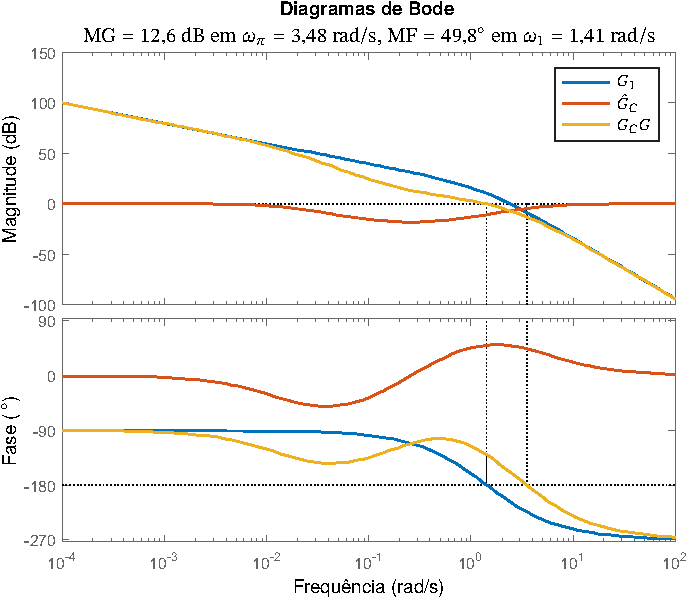
\includegraphics[scale=1]{bodediagram.pdf}
\end{figure}

Para manter a coerência no uso de software livre (já que você está usando \LaTeX), teste a ferramenta \textsf{InkScape} (\url{http://inkscape.org/}). Ela é uma excelente opção de código-livre para produzir ilustrações vetoriais, similar ao CorelDraw ou ao Adobe Illustrator.

De todo modo, caso não seja possível utilizar arquivos de imagens como \texttt{pdf}, utilize qualquer outro formato, como \texttt{jpeg}, \texttt{gif} e \texttt{bmp}. Estes formatos requerem maior tempo de processamento, mas você pode tentar aprimorar seus conteúdos com o software livre \textsf{Gimp} (\url{http://www.gimp.org/}), uma alternativa livre ao Adobe Photoshop. A \cref{fig:logolatex} mostra como é fácil inserir uma figura com legenda e referência à fonte utilizando um arquivo no formato \texttt{png}.

\begin{figure}[htb]
    \begin{center}
    \caption{Logo \LaTeX} \label{fig:logolatex}
    
\includegraphics[width=0.5\linewidth]{1280px-LaTeX-logo.png}
    \captionsetup{aboveskip=0pt,belowskip=2pt}
    \fonte{Wikimedia Commons \cite{wikimedia-latex}}
    \end{center}
\end{figure}

Também é possível criar figuras, diagramas e gráficos utilizando comandos de pacotes disponíveis para o \LaTeX, como \textsf{TikZ}. Entretanto, tais pacotes requerem elevado tempo de processamento no Overleaf e, por isso, não foram utilizados neste documento.

Note que, de acordo com as normas da ABNT, numeração e título das figuras e tabelas devem aparecer na parte superior. Na parte inferior deve ser informada a fonte.

% ---
\subsection{Figuras em \emph{minipages}}
% ---

\emph{Minipages} são usadas para inserir textos ou outros elementos em quadros com tamanhos e posições controladas. Veja os exemplos das \cref{fig:minipage_circuito,fig:minipage_grafico}.

\begin{figure}[htb]
    \label{fig:teste}
    \centering
    \begin{minipage}[t]{0.46\textwidth}
        \centering
        \caption{Imagem da minipage}
        \label{fig:minipage_circuito}
        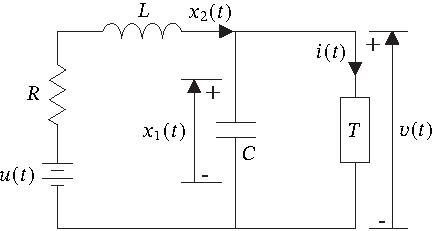
\includegraphics[scale=1]{circuito.pdf} 
    \end{minipage}
    \hfill
    \begin{minipage}[t]{0.52\textwidth}
        \centering
        \caption{Gráfico da minipage}
        \label{fig:minipage_grafico}
        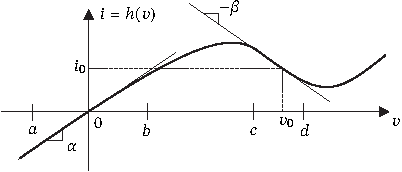
\includegraphics[scale=1.2]{diodocurva.pdf}
    \end{minipage}
\end{figure}

\subsection{Subfiguras}

O pacote \textsf{subfig} foi utilizado para inserir as \cref{fig:subfigura_circuito,fig:subfigura_grafico}. Subfiguras também podem ser inseridas no texto com o pacote \textsf{subcaption}.

% utiliza o pacote subfig
\begin{figure}[htb]
    \centering
    \caption{Figura com subfiguras}
    \label{fig:subfiguras}
    \subfloat[Primeira subfigura]{\label{fig:subfigura_circuito} \centering 
    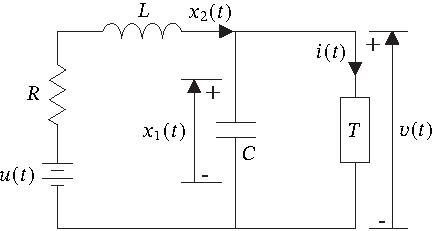
\includegraphics[scale=1]{circuito.pdf}} 
    \subfloat[Segunda subfigura]{\label{fig:subfigura_grafico} \hspace{0.4em}
    \centering 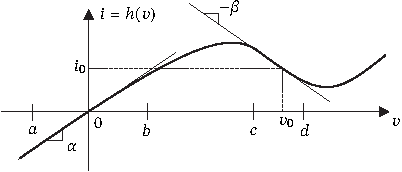
\includegraphics[scale=1.2]{diodocurva.pdf}}
\end{figure}

% utiliza o pacote subcaption
%\begin{figure}[htb]
%    \centering
%    \caption{Figura com subfiguras}
%    \label{fig:subfiguras}
%    \begin{subfigure}[t]{0.47\textwidth}
%        \caption{Primeira subfigura}
%        \label{fig:subfigura_circuito}
%        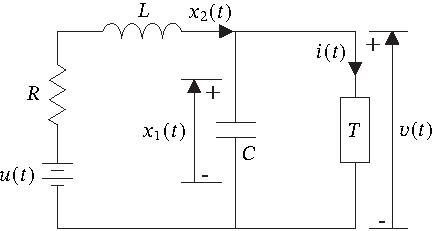
\includegraphics[scale=1]{circuito.pdf}
%    \end{subfigure}%
%    \hfill
%    \begin{subfigure}[t]{0.52\textwidth}
%        \caption{Segunda subfigura}
%        \label{fig:subfigura_grafico}
%        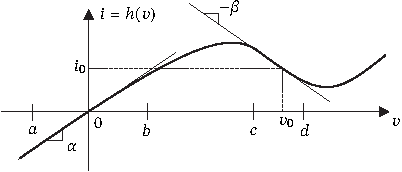
\includegraphics[scale=1.2]{diodocurva.pdf}
%    \end{subfigure}
%\end{figure}

% ---
\subsection{Figuras que usam as mesmas fontes tipográficas do documento}
% ---

Caso queira utilizar as mesmas fontes tipográficas do texto para escrever dentro de figuras, como é o caso da \cref{fig:psfrag1} (arquivo \texttt{blockdiagram.pdf}), produza uma figura como a da \cref{fig:psfrag2} e a salve no formato \texttt{eps} (arquivo \texttt{blockdiagram.eps}). Softwares como InkScape, CorelDraw ou Adobe Ilustrator podem ser utilizados para este fim.

\begin{figure}[htb]
    \centering
    \caption{Uso do pacote \textsf{psfrag}}
    \subfloat[Arquivo \texttt{blockdiagram.pdf}]{\label{fig:psfrag1} \centering 
    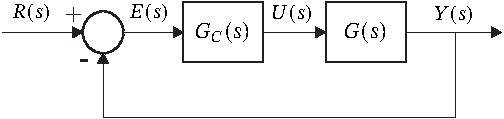
\includegraphics[scale=1]{blockdiagram.pdf}}  \\
    \subfloat[Arquivo \texttt{blockdiagram.eps}]{\label{fig:psfrag2}
    \centering 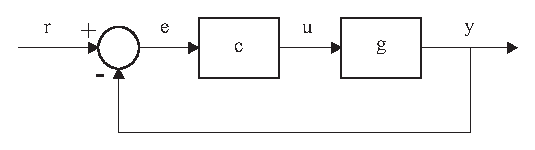
\includegraphics[scale=1]{blockdiagram.eps}}
    \label{fig:psgrag}
\end{figure}

Crie no Overleaf um novo projeto que tenha o conteúdo do \cref{cod:tex} dentro de um arquivo \texttt{tex} nomeado, por exemplo, como \texttt{blockdiagram.tex}. No menu do Overleaf, altere o compilador de \texttt{pdfLaTeX} para \texttt{LaTeX} e defina o arquivo \texttt{blockdiagram.tex} como principal. Coloque o arquivo \texttt{blockdiagram.eps} dentro do projeto e compile. A saída gerada, corresponde à \cref{fig:psfrag1}, deve ser salva como \texttt{blockdiagram.pdf}. Este arquivo poderá ser carregado no projeto do texto do trabalho (TCC, dissertação ou tese) que você estiver escrevendo com o UnB\TeX\ (que usa o \texttt{pdfLaTeX} como compilador).

\lstinputlisting[numbers=none,float,caption={\texttt{blockdiagram.tex}},label={cod:tex}]{unbtex-example/codigos/blockdiagram.tex}

Observe na \cref{fig:psfrag2} que o ``\texttt{g}'' é substituído por ``$G(s)$'' na \cref{fig:psfrag1}. Para tal, o \cref{cod:tex} utiliza o seguinte comando do pacote \textsf{psfrag}:
\begin{verbatim}
\psfrag{g}[c][c]{\footnotesize $G(s)$}
\end{verbatim}

O pacote \textsf{psfrag} funciona apenas com o compilador \texttt{LaTeX}, o que torna a criação de um novo projeto no Overleaf uma boa solução. Este projeto poderá ser aproveitado para gerar outras figuras do documento principal. Para mais informações sobre o pacote, consulte seu manual\footnote{Disponível em \url{http://mirrors.ctan.org/macros/latex/contrib/psfrag/pfgguide.pdf}}.

Evite o uso de figuras no formato \texttt{eps} no documento principal. Documentos que usam a classe UnB\TeX\ precisam ser compilados pelo \texttt{pdfLaTeX}, que inicialmente converte os arquivos \texttt{eps} para o formato \texttt{pdf}, exigindo maior tempo de processamento. O projeto auxiliar (\cref{cod:tex}) usa a classe \texttt{article} e admite compilador \texttt{LaTeX}, que não necessita de etapas adicionais para processar códigos que chamam arquivos \texttt{eps}.